\documentclass[a4paper, twocolumn]{article}
\usepackage{graphicx} % Required for inserting images

\title{Predicting Fuel Efficiency of Cars using Linear and Logistic Regression}
\author{M. Fjeldberg, M. Svensson}
\date{March 2026}

\begin{document}

\maketitle

\begin{abstract}
In this project we explore the use of linear regression to predict the miles per gallon (MPG)
of cars based on their physical attributes. We also investigate whether regularisation techniques (Ridge and Lasso regression) can improve the model's performance. We evaluate the models using common regression metrics and compare the results to determine the effectiveness of regularisation on this dataset.
\end{abstract}

\section{Introduction}

In this project we look at how well a simple machine learning model can predict the fuel efficiency of a car.
We use the carssplit.csv dataset, which contains information about 398 cars from the 1970s and 1980s, including attributes like weight, horsepower, number of cylinders and model year.

The goal is to answer a straightforward question: given a car's physical specifications, can we predict how many miles per gallon it gets?
To do this we train a linear regression model and then try to improve it by fine-tuning with regularisation techniques (Ridge and Lasso regression).

We evaluate the models using common regression metrics such as Mean Absolute Error (MAE), Root Mean Square Error (RMSE) and R², and compare the results to see whether regularisation helps on this particular dataset.

\section{Method}

The dataset contains 398 entries, but 6 rows have missing values for horsepower. We drop these, leaving 392 usable rows. We select seven numeric features as input: cylinders, displacement, horsepower, weight, acceleration, model year and origin. The target variable is MPG.

We split the data into 80\% training and 20\% test sets and standardise all features using \texttt{StandardScaler} so that each feature has zero mean and unit variance. This ensures that no single feature dominates the model due to its scale.

We first train a baseline ordinary least-squares (OLS) linear regression model. Linear regression fits a set of weights to the features that minimises the sum of squared errors between predicted and actual MPG values.

To fine-tune, we try two regularised variants:
\begin{itemize}
    \item \textbf{Ridge regression} adds an L2 penalty that shrinks coefficients toward zero, reducing overfitting.
    \item \textbf{Lasso regression} adds an L1 penalty that can shrink some coefficients all the way to zero, effectively performing feature selection.
\end{itemize}

For both Ridge and Lasso we test five alpha values (0.01, 0.1, 1.0, 10.0, 100.0) using 5-fold cross-validation on the training set and pick the alpha with the highest mean R². The best model is then evaluated on the held-out test set.

\section{Results}

The baseline linear regression model achieves an MAE of 2.42, RMSE of 3.27 and R² of 0.790 on the test set. This means the model explains about 79\% of the variance in MPG.

After cross-validation, the best Ridge alpha was 1.0 and the best Lasso alpha was 0.1. Table~\ref{tab:comparison} shows that regularisation did not improve performance — the plain OLS model performs marginally best.

\begin{table}[h]
\centering
\small
\begin{tabular}{lccc}
\hline
\textbf{Model} & \textbf{MAE} & \textbf{RMSE} & \textbf{R²} \\
\hline
Linear Reg. & 2.42 & 3.27 & 0.790 \\
Ridge ($\alpha$=1.0) & 2.42 & 3.28 & 0.789 \\
Lasso ($\alpha$=0.1) & 2.42 & 3.30 & 0.786 \\
\hline
\end{tabular}
\caption{Model comparison on the test set.}
\label{tab:comparison}
\end{table}

The feature coefficients show that \textit{weight} has the strongest negative effect on MPG, while \textit{model year} has the strongest positive effect — lighter and newer cars are more fuel-efficient.

Figure~\ref{fig:actual_vs_pred} shows that predictions track the actual values well, though the model underestimates some high-MPG cars.

\begin{figure}[h]
\centering
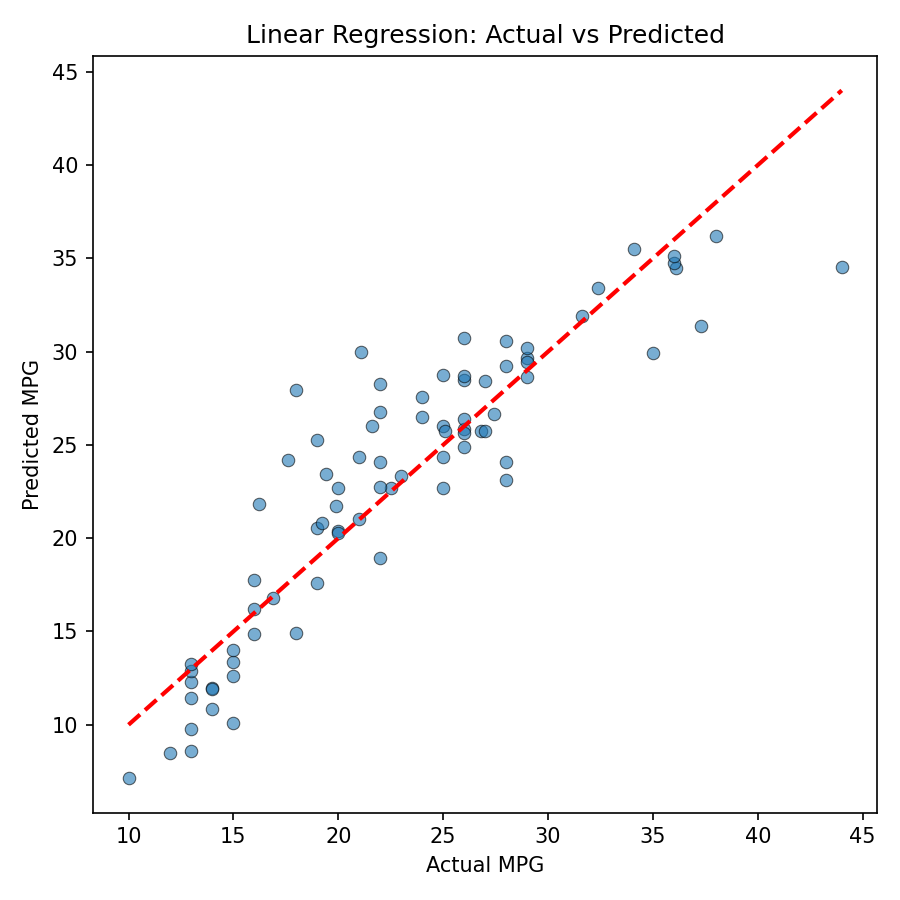
\includegraphics[width=\columnwidth]{images/actual_vs_predicted.png}
\caption{Actual vs predicted MPG for the baseline linear regression model.}
\label{fig:actual_vs_pred}
\end{figure}

\section{Conclusion}

\end{document}
